% chapters/ch3-sec7.tex -- 7. Model Rocket Drag at Transonic and Supersonic Speeds;
% 7.1 Limits on the Applicability of Incompressible Analysis; 7.2 Drag Divergence;
% 7.3 Semiempirical Determination of Transonic and Supersonic Drag Coefficients
% (PDF 505-516, printed pp. 473-484)
\section{Model Rocket Drag at Transonic and Supersonic Speeds}\label{ch3:sec:7}

\subsection{Limits on the Applicability of Incompressible Analysis}\label{ch3:sec:7.1}

As stated in Section~\ref{ch3:sec:2.1.1}, the results of the analyses
and semiempirical treatments contained in the first six sections
of this chapter can be assumed accurate on an \emph{a priori} basis
only if the compression of the atmosphere due to the airspeed
of the model is relatively slight. The reader may also recall
from this discussion that the analytical criterion of ``sufficiently
slight'' compression corresponds to a \emph{Mach number} $M$ of less than
0.316, where
\begin{equation}\label{ch3:eq:212}
M = \frac{U_\infty}{c}
\end{equation}
and $c$ is the speed with which sound waves travel through the
air: the so-called ``speed of sound''.

Strictly speaking, the Mach number associated with a given
airspeed varies with atmospheric conditions, since $c$ itself
varies with atmospheric composition and temperature. In this
connection you may again wish to consult Figure~\ref{ch3:fig:4}, which shows
the variation of sound speed with altitude for the United States
standard atmosphere. The dependence of $c$ upon local temperature
is given by
\begin{equation}\label{ch3:eq:213}
c = c_{\mathrm{std}}\sqrt{\frac{T}{T_{\mathrm{std}}}}
\end{equation}
where $T_{\mathrm{std}}$ is the standard atmospheric temperature at the altitude
in question and $T$ is the actual temperature at that altitude
at the time in question, and where the temperatures must be
measured on one of the absolute scales, Rankine or Kelvin.
It is found from Figure~\ref{ch3:fig:4} and equation~\eqref{ch3:eq:213}, however, that
the speed of sound varies only slightly---a few percent at
most---over the range of temperatures for which it is practical
to launch model rockets and over the range of altitudes present-day
models can achieve. It is therefore reasonable to assume
that $c$ remains constant at its sea-level standard value of
about 340 meters/second for all calculations of interest to
model rocketeers. The maximum airspeed at which the results
obtained from incompressible-flow theory can be considered
analytically valid is therefore approximately 107 meters/second.

Above this speed the influence of compressibility on the
flow about the rocket makes its presence known through a number
of phenomena. The air in the vicinity of the stagnation points
at the tip of the nose and the leading edges of the fins, as
well as the air within the boundary layer, increases noticeably
in density. The boundary layer thickens and its velocity
profile becomes altered. The fins behave as if their aspect
ratio were lower than that which is geometrically the case. A
precise, analytical description of the effects of each of these
phenomena upon the overall drag of the model would fill a
book by itself. It is not our purpose to present such a treatment
here, as the mathematics involved are quite a bit more complex
than those by which we have been able to treat incompressible
flow. Furthermore, only a small portion of the vast literature
that has grown up around the study of compressible fluid flow
is of appreciable interest to model rocketeers. What \emph{is} of
interest to us as designers of high-performance model rockets
is the experimentally-observed fact that \emph{the overall drag
coefficient of a finned body of revolution, such as a model
rocket, does not exhibit any appreciable deviation from the value
predicted by incompressible flow theory at Mach numbers below
0.9}. It is Nature's gift to the designer that the various
compressibility phenomena interact in such a manner as to make
this true. Although the results of incompressible flow theory
are not \emph{analytically valid} above $M = 0.316$, therefore, they
are \emph{numerically accurate} up to $M = 0.9$ and may thus be used
without modification in closed-form performance calculations.
In short, the effects of compressibility on the drag coefficient
of a model rocket are negligible at airspeeds up to approximately
306 meters/second.

\subsection{Drag Divergence}\label{ch3:sec:7.2}

As a model rocket approaches ``Mach one''---the speed of
sound---regions form near the nose tip and the fin leading
edges in which the air is highly compressed over a relatively
short distance. In a similar manner, regions form near the
fin trailing edges and the body tube base in which the air
expands again to fill the partial void left by the rocket's
passage. This behavior is associated with the fact that the
speed of sound in a fluid is \emph{the speed with which fluid elements
can transmit information to one another}. As a body travelling
through the fluid approaches the sonic velocity the fluid directly
in front of it cannot ``inform'' the fluid further upstream that
the body is approaching in time for the upstream fluid elements
to move smoothly aside to let the body pass (as they do in subsonic
flight). The upstream elements therefore ``pile up'' on one
another and become crushed, or compressed, against the nose
tip and the fin leading edges of a model rocket entering the
transonic flight regime. Once the model has passed by, the
compressed fluid elements endeavor to return to their original
volume, thus undergoing a rapid expansion.

At a Mach number of 1.0 the region of compression at the
nose becomes a thin surface normal to the longitudinal axis
of the rocket, called a \emph{normal shock}. As $M$ increases above 1.0
the compression region becomes conical, with the cone half-angle
decreasing as the Mach number increases: a three-dimensional
\emph{oblique shock}. The surface bounded by the oblique shock trailing
from the nose of a supersonically-flying body of revolution is
called the \emph{Mach cone}; in cases of horizontally-flying airplanes
this cone may intersect the ground, causing observers to hear
the so-called \emph{sonic boom}. In addition, any sound produced by
the body itself can only be heard within the Mach cone; to an
observer outside the cone the vehicle appears to be flying in
perfect silence. For this reason a supersonic airplane can
only be heard after it has already passed overhead, and an
observer on the ground must ``lead'' the sound (i.e., look ahead
of it) in order to see the aircraft. The expansion of the
atmosphere into the region behind a model rocket in supersonic
flight occurs with a very rapid decrease in density, exhibiting
a characteristic flow pattern known as the \emph{Prandtl-Meyer expansion
fan}.

Now the importance of these phenomena to model rocket drag
is that the air which passes through the shock and expansion
pattern surrounding the model is \emph{not} returned completely to
its original state once the rocket has gone by. The shock/expansion
system causes a certain amount of \emph{momentum} to be transferred
from the model to the airstream over and above the quantity
that would be transferred under subsonic conditions. The drag
coefficient of a model rocket in transonic and supersonic flight
is therefore \emph{greater} than its subsonic drag coefficient.
Typically, $\CD$ increases rapidly as Mach 1.0 is approached,
reaches a peak at slightly above the sonic velocity, and declines
again toward a value that is somewhat greater than the subsonic
drag coefficient as the Mach number increases toward 2.0. The
rapid increase experienced in the transonic regime, between
$M = 0.9$ and the Mach number at which the peak $\CD$ occurs, is
called \emph{drag divergence}. The existence of drag divergence is
one reason that it was common to call Mach one ``the sound barrier''
before the rocket-powered Bell X-1 airplane first exceeded it
in 1947, and for some years thereafter. Drag divergence also
means that it is extremely difficult for small vehicles of
limited total impulse, such as model rockets, to exceed Mach
one. Only our very highest-performance designs can accomplish
this feat, and then only when powered by the highest-thrust
model rocket engines available---types B14, F67, F100, and
so on---and even then resort must often be had to multiple
staging.

\subsection{Semiempirical Determination of Transonic and Supersonic Drag Coefficients}\label{ch3:sec:7.3}

The mathematical complexity associated with the analysis
of compressible fluid flow about a finned body of revolution
is too great to permit the practical calculation of transonic
and supersonic drag coefficients directly from first principles.
As was the case for subsonic flight, we must have recourse to
semiempirical formulae based on experimental data in order to
obtain values of $\CD$ for use in model rocket performance calculations.
Hoerner~(\ref{ch3:ref:9}) presents drag coefficient data for a number of
small fin-body combinations tested at transonic and supersonic
velocities. As shown in Figure~\ref{ch3:fig:53}a, the test results fall into
two distinct categories: one containing rockets having sharp
(ogival or conical) noses, and one comprised of models having
rounded nose shapes. For the sharp-nosed rockets the drag
coefficient $\CD$ rises to 1.7 times its subsonic value (denoted
$C_{Ds}$) at $M = 1.05$ and then declines again to about $1.27\,C_{Ds}$
as $M$ approaches 2.0. The round-nosed configuration is more
severely affected by compressibility: its $\CD$ peaks at $2.17C_{Ds}$
at $M = 1.2$ and falls back only as far as $2.0C_{Ds}$ for $M$ approaching
2.0. The difference in behavior between the two configuration
classes is due to a fundamental difference in nature between
the shock associated with a sharp nose and the shock generated
by a rounded nose. The oblique shock produced by a sharp nose
in supersonic flight is an \emph{attached} shock; i.e., the shock
appears to be shed directly from the point of the nose like a
cone suspended on a pencil point. The shock due to a rounded
nose, on the other hand, is itself rounded at its forward
extremity and is \emph{detached}: it ``stands off'' slightly ahead of
the front surface of the nose itself. Figure~\ref{ch3:fig:54} illustrates
the difference in structure between the two shock patterns,
and also the shock/expansion pattern observed in the neighborhood
of the base of a blunt-based body of revolution. As there is
appreciably greater momentum transfer associated with the
detached than with the attached shock, the rounded-nose configurations
have higher drag coefficients at transonic and supersonic
velocities.

\begin{figure}[htbp]
  \centering
  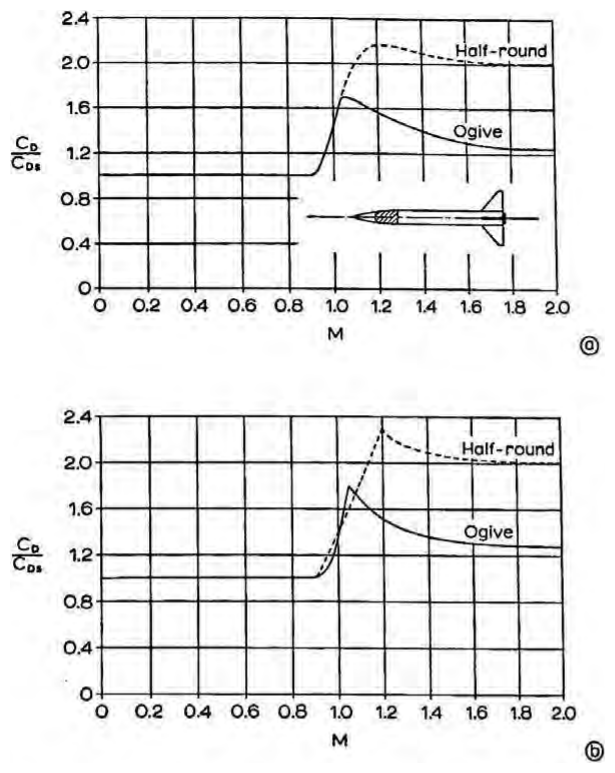
\includegraphics[width=0.7\textwidth,height=0.7\textheight,keepaspectratio]{figures/ch3/fig53.png}
  \caption{Variation of drag coefficient with Mach number for
  finned bodies of revolution. (a): Experimentally determined
  behavior of the drag coefficient of the rocket pictured, using
  both ogive and half-round noses. (b): Analytical functions
  described in equations~\eqref{ch3:eq:214} and~\eqref{ch3:eq:215} that approximate the
  experimental behavior to within 10\%.}
  \label{ch3:fig:53}
\end{figure}

\begin{figure}[htbp]
  \centering
  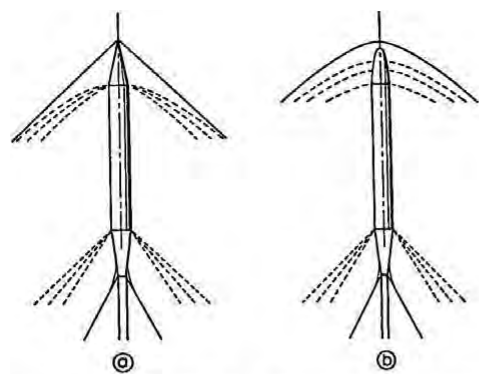
\includegraphics[width=0.6\textwidth,height=0.85\textheight,keepaspectratio]{figures/ch3/fig54.png}
  \caption{Shock and expansion patterns about sharp-nosed and
  blunt-nosed bodies of revolution. Solid lines indicate shocks
  and compression waves; dotted lines indicate expansion waves or
  fans; wavy lines delineate the wakes of the bodies. The conical
  nose produces an attached shock (a) which results in a lower drag
  than the detached shock (b) formed in front of the rounded nose.}
  \label{ch3:fig:54}
\end{figure}

It is mathematically possible to construct formulae for
the drag coefficients which will represent the curves of Figure~\ref{ch3:fig:53}a
to a very high order of precision. Such a procedure is
not really worth the trouble, though, since the data presented
in Figure~\ref{ch3:fig:53}a are only approximate (in fact, the curves above
Mach 1.5 are based on extrapolation) and their applicability to
a wide range of model rocket configurations has not been established.
If one takes the liberty of initially assuming a high-performance
rocket configuration (which in itself is justified by the fact
that only the highest-performance model rockets are in fact
capable of exceeding Mach one), however, it should prove possible
to construct approximating functions that are relatively simple,
yet will represent $\CD$ with reasonable accuracy over the Mach
number range of interest to the hobbyist.

One possible choice for such a function assumes a rise in
$\CD$ given by a power function in Mach number, followed by a
decline given by an exponential in Mach number. Such a representation
is referred to as \emph{piecewise smooth}, since the graph
obtained from such a set of formulae is a smooth curve everywhere
except at the point at which the first formula leaves off and
the second begins---where there is a sharp ``peak''. It will
be found that a reasonably accurate set of approximating functions
of this type for sharp-nosed vehicles is given by
\begin{subequations}\label{ch3:eq:214}
\begin{align}
\frac{\CD}{C_{Ds}} &= 1.0 + 35.5\,(M - 0.9)^{2}
  &&(0.9 \le M \le 1.05) \label{ch3:eq:214a}\\
\frac{\CD}{C_{Ds}} &= 1.27 + 0.53\,e^{-5.2(M - 1.05)}
  &&(1.05 \le M \le 2.0) \label{ch3:eq:214b}
\end{align}
\end{subequations}
and that a similar set for round-nosed rockets may be written
\begin{subequations}\label{ch3:eq:215}
\begin{align}
\frac{\CD}{C_{Ds}} &= 1.0 + 4.88\,(M - 0.9)^{1.1}
  &&(0.9 \le M \le 1.2) \label{ch3:eq:215a}\\
\frac{\CD}{C_{Ds}} &= 2.0 + 0.3\,e^{-5.75(M - 1.2)}
  &&(1.2 \le M \le 2.0) \label{ch3:eq:215b}
\end{align}
\end{subequations}
These approximating functions are displayed in Figure~\ref{ch3:fig:53}b and
compared with the experimental data curves in Table~\ref{ch3:tab:8}. Inspection
of Table~\ref{ch3:tab:8} reveals that even these relatively simple functions
predict $\CD$ values within 10\% of those determined by experiment
over the Mach number range 0.9 through 2.0.

\begin{table}[htbp]
  \centering
  \caption{Comparison of the analytical drag divergence functions
  $(\CD/C_{Ds})_a$ given in equations~\eqref{ch3:eq:214} and~\eqref{ch3:eq:215} with the experimentally
  observed drag divergence functions $(\CD/C_{Ds})_e$ for rockets with
  ogive and half-round noses at Mach numbers between 0.9 and 2.0.}
  \label{ch3:tab:8}
  Ogive Nose\par\smallskip
  \begin{tabular}{@{}S[table-format=1.2] S[table-format=1.2] S[table-format=1.3] S[table-format=-1.2]@{}}
    \toprule
    {$M$} & {$\left[\dfrac{\CD}{C_{Ds}}\right]_e$} & {$\left[\dfrac{\CD}{C_{Ds}}\right]_a$}
      & {\begin{tabular}{@{}c@{}}Percent\\ error\end{tabular}} \\
    \midrule
    0.90 & 1.00 & 1.000 & 0.00 \\
    0.95 & 1.17 & 1.089 & -6.92 \\
    1.00 & 1.43 & 1.355 & -5.25 \\
    1.05 & 1.70 & 1.800 & 5.56 \\
    1.10 & 1.67 & 1.680 & 0.60 \\
    1.20 & 1.57 & 1.513 & -3.63 \\
    1.40 & 1.40 & 1.356 & -3.14 \\
    1.60 & 1.30 & 1.300 & 0.00 \\
    1.80 & 1.27 & 1.281 & 0.84 \\
    2.00 & 1.27 & 1.274 & 0.31 \\
    \bottomrule
  \end{tabular}

  \bigskip
  Half-Round Nose\par\smallskip
  \begin{tabular}{@{}S[table-format=1.2] S[table-format=1.2] S[table-format=1.3] S[table-format=-1.2]@{}}
    \toprule
    {$M$} & {$\left[\dfrac{\CD}{C_{Ds}}\right]_e$} & {$\left[\dfrac{\CD}{C_{Ds}}\right]_a$}
      & {\begin{tabular}{@{}c@{}}Percent\\ error\end{tabular}} \\
    \midrule
    0.90 & 1.00 & 1.000 & 0.00 \\
    0.95 & 1.17 & 1.182 & 1.03 \\
    1.00 & 1.43 & 1.389 & -2.86 \\
    1.05 & 1.76 & 1.610 & -8.50 \\
    1.10 & 2.00 & 1.830 & -8.50 \\
    1.20 & 2.17 & 2.300 & 6.00 \\
    1.40 & 2.10 & 2.095 & -0.24 \\
    1.60 & 2.03 & 2.030 & 0.00 \\
    1.80 & 2.00 & 2.010 & 0.48 \\
    2.00 & 2.00 & 2.003 & 0.15 \\
    \bottomrule
  \end{tabular}
\end{table}

I cannot emphasize strongly enough, however, that you
should \emph{not} regard equations~\eqref{ch3:eq:214} and~\eqref{ch3:eq:215} as having any valid
basis in mathematical physics, or as having a precision anywhere
near that of the \emph{Datcom} equations for subsonic flight. The
tenuous nature of the connection between the experimental data
and the actual flight of model rockets, and the extent to which
I have extrapolated the data curves, is such that the best that
can be said of equations~\eqref{ch3:eq:214} and~\eqref{ch3:eq:215} is that they represent
\emph{reasonable suggestions} of the behavior of model rocket drag
coefficients at transonic and supersonic speeds. They are to
be used with the understanding that they are tentative and
with the provision that they are acceptable for use only until
better approximations are available. At present, however,
they may be considered accurate enough for design study and
altitude prediction work.

Finally, the reader should realize that the behavior of
the drag coefficient at these high velocities presents us with
a fundamental analytical difficulty in carrying out performance
calculations. Since $\CD$ in this flight regime is a strongly-varying
function of Mach number, and hence of velocity, a
constant, average value of $\CD$ \emph{cannot} be used in computing
altitude performance. This precludes the use of any of the
closed-form, analytical altitude-performance equations presented
in Chapter~\ref{ch4} and makes the use of computerized interval methods
essential in calculating the performance of any model rocket
that is expected to enter the transonic and/or supersonic
range of velocities at any time during its flight.
